% !TEX root = ../ClassicThesis_DEIB.tex

\chapter{The Robì project} \label{chap:robìProject}

A branch of this thesis work involved the customization of the prototype mobile manipulator Robì \parencite{robi} to the requirements of the mobile base requested by the \ac{GRAPE} project. 


\begin{figure}
	\centering
	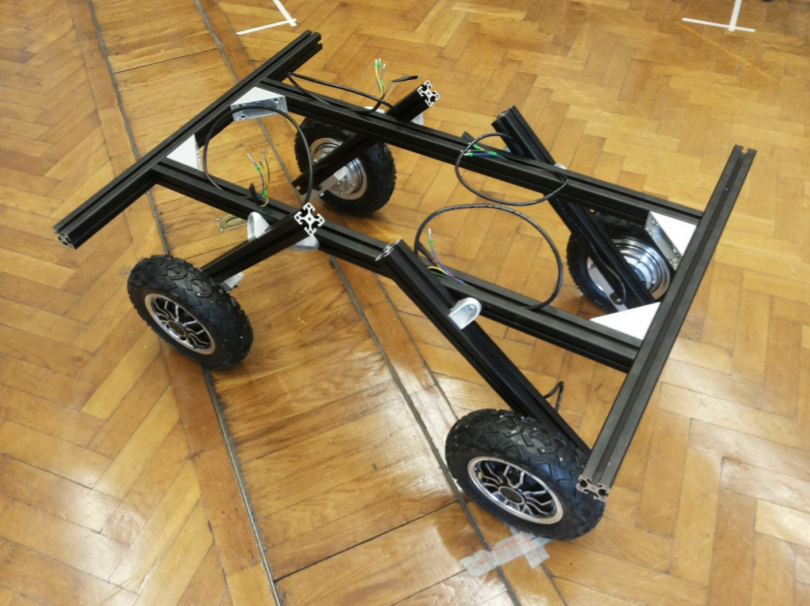
\includegraphics[width=0.6\textwidth]{Images/robi/robi_inizio.png}
	\caption{\textit{The Robì mobile manipulator chassis, in one of its}}
	\label{fig:robiDefault}
\end{figure}


\section{Robì mobile manipulator}
Robì (see Figure \ref{fig:robiDefault}) is a prototype small-sized mobile manipulator for agricultural applications, whose aim is to support the development and testing of innovative perception and control algorithms. Both the mechanical structure and the motion control system are designed to be simple, flexible, low-cost and low-weight, to create a system that can act as an open source base for project in agricultural robotics, contrary to the large amount of task-specific platforms in agricultural robotics (\textit{e.g.} for asparagus \parencite{asparagi} or tomato \parencite{pomodori} harvesting).

\par Since the platform is thought as a versatile mobile base to be adapted to several fields (\textit{e.g.} vineyards, herbaceous plants) its chassis is designed to have flexible geometrical characteristics (ground clearance, track, wheelbase).

 \begin{table}[tb]
\footnotesize
\centering
\begin{tabularx}{0.45\textwidth}{ll}
\toprule
\tablefirstcol{l}{Ground clearance}
& [0.25, 0.35] m \\
\tablefirstcol{l}{Track}
& [0.75, 1.2] m \\
\tablefirstcol{l}{Wheelbase}
& [0.6, 1] m \\
\toprule
\end{tabularx}
\caption[Ranges of Robì geometrical characteristics]{\textit{Ranges of Robì geometrical characteristics.}}
\label{tab:robiConfiguration}
\end{table}

 More generally, the design principles of Robì are:
 
\begin{itemize}
	\item \textbf{low cost}, to make it easier to use it for example applications and, possibly, fleet-based applications
	\item \textbf{low weight}, to increase the battery life and, consequently, allow for more long and versatile missions
	\item \textbf{simple mechanical design}, to make it easy to build it out of a mounting kit
\end{itemize}

\begin{figure}
	\centering
	\subfloat[]{%
		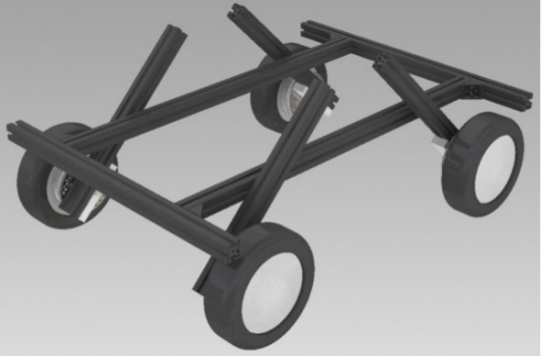
\includegraphics[width=0.45\textwidth]{Images/robi/robi_config1.png}
		\label{fig:robiConfig1}}
	\qquad
	\subfloat[]{%
		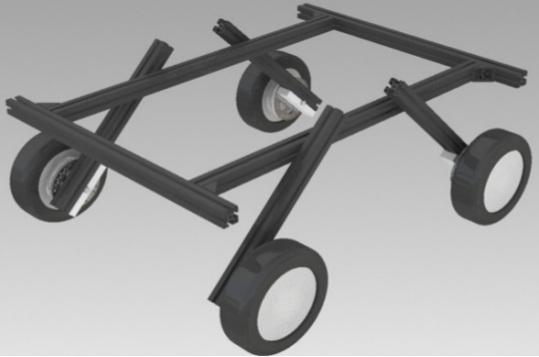
\includegraphics[width=0.45\textwidth]{Images/robi/robi_config2.png}
		\label{fig:robiConfig2}} \\
	\subfloat[]{%
		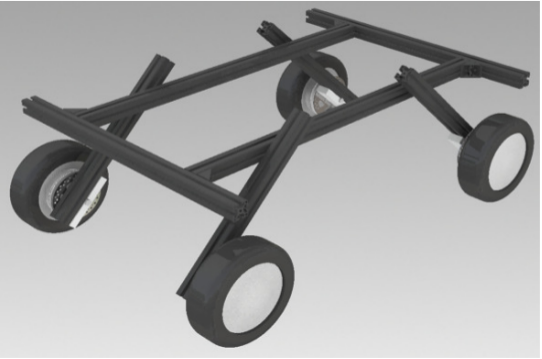
\includegraphics[width=0.45\textwidth]{Images/robi/robi_config3.png}
		\label{fig:robiConfig3}}
	\caption{\textit{3D rendering of different configuration of Robì base, obtained thanks to the chassis mechanical design.}}
	\label{fig:robiConfigurations}
\end{figure}

The aforementioned principles are implemented through the following design choices:
\begin{description}
	\item[Chassis] \hfill \\ The chassis is made out of ITEM\textsuperscript{\textregistered} aluminium bars, that presents lightweight but strong section; the slide rails embedded in the ITEM\textsuperscript{\textregistered} bars, together with four rotational joints applied to the bars supporting the wheels, allow for multiple configuration of the robot geometrical characteristics to vary in the ranges listed in Table \ref{tab:robiConfiguration}. In Figure \ref{fig:robiConfigurations} you can see 3D rendering of some of the available Robì configurations. The bars that support the wheel, however, can't rotate during the robot movement, thus Robì has a skid steering kinematic model.
	
	\item[In-wheel motors] \hfill \\ Robì is powered by four in-wheel electric DC brushless motors; the model is HUB10GL (see Figure \ref{fig:robiMotori}). In-wheel motors have been chosen mostly because they allow for much simpler mechanical design, with respect to classical electrical powertrain, because:
	\begin{itemize}
		\item no transmission is required
		\item the weight is reduced, and the available space on the chassis increases
		\item high level of maneuverability, without the need to introduce Ackermann kinematics
	\end{itemize}
	The motors are independent, so a suitable control board is required to control each of them; the board used in Robì are the ones described in VESC project\footnote{\url{http://vedder.se/2015/01/vesc-open-source-esc/}},
an open source brushless motor control project. These boards offers several interfaces to control the motor:  PPM signal, analog, UART, I$^2$C, USB  or CAN-bus.
\end{description}

\begin{figure}
	\centering
	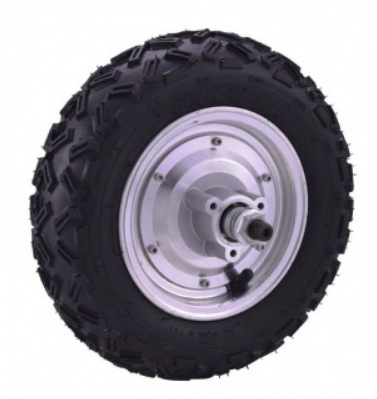
\includegraphics[width=0.4\textwidth]{Images/robi/motore.png}
	\caption{\textit{HUB10GL, the in-wheel motor model adopted in Robì.}}
	\label{fig:robiMotori}
\end{figure}

\section{Robì as GRAPE mobile base}
The features mentioned in the previous section made RObì a convincing candidate as the mobile platform for the \ac{GRAPE} project, because of its flexibility as a mobile manipulator for agricultural robotics field. Unfortunately, for mere lack of time, in the late phases the project focused on the development of the whole system on a commercial robot, the Husky that was already described as the final \ac{UGV} of the \ac{GRAPE} project.
\par However, significant steps in the adaptation of Robì as a base for a real agricultural robotic project were made, thus we are explaining them in this section.

\subsection{Hardware configuration}
Since the idea was to replicate the configuration of the Husky platform for the \ac{GRAPE} project, similar sensors were mounted on it; on the other side, we had to dedicate significant efforts to the creation of an hardware interface between the on-board computer (a commercial HP laptop) to the motors control board.

\begin{itemize}
	\item architettura hw: sensori che ci sono montati a bordo, spiegazione sistema controllo motori tramite CAN usando la board STM
	\item architettura sw: compatibile con quella di Grape, a meno dei nodi driver dei sensori e attuatori
	\item spiegazioni e immagini del vario hardware
\end{itemize}
